\chapter{INTRODUÇÃO}\label{ch:introducao}

Redes sociais se tornaram um termo comum e uma chave fundamental para o estilo de vida moderno. Hoje em dia, a maioria das pessoas, independente de idade, sexo, crença, utilizam uma ou mais redes sociais. A princípio, esses ambientes \textit{on-line} focavam-se na comunicação, por exemplo; a possibilidade de se comunicar com alguém distante e tornar esse diálogo pessoal, seguro e, de alguma forma, próximo, ajudando na popularização desse tipo de tecnologia. No decorrer dos anos e com o avanço tecnológico, diferentes tipos de redes sociais surgiram com ideias semelhantes ou extremamente diferentes, não sendo apenas para a comunicação, mas para outros fins como o compartilhamento de mídias, localização, críticas, \textit{mini-blogs}, perguntas e respostas, negócios, profissão, música, artes, venda e troca de produtos, entre outros.

\textit{Facebook}, \textit{Twitter}, \textit{LinkedIn}, \textit{Google+} e, muito comum entre desenvolvedores, o \textit{GitHub} são exemplos populares de redes sociais. Logo, possuem grande número de usuários e diversas interações que estes realizam a cada momento, gerando uma quantidade gigantesca de dados. Devido a diversidade e a vasta quantidade de informação gerada, algumas redes sociais podem utilizá-las para o aprimoramento de conteúdo ou, então, para o comércio de dados para empresas, por exemplo; publicidade e marketing, que fazem a mineração desses dados para encontrar padrões de seus usuários e, assim, conseguir aumentar suas vendas, reduzir riscos e, até mesmo, gerar novas tendências.

Nesse sentido, dados é um termo deliberadamente vago, que agrega várias formas comuns de informações, como matrizes (vetores multidimensionais), planilhas ou tabelas, em que cada coluna pode ter um tipo diferente de informação: caracteres, numéricos, data, entre outros. As tabelas, por sua vez, também podem se relacionar através de colunas apresentadas no tradicional modelo de bancos de dados relacionais. Todavia, não é sempre que um percentual de um conjunto de dados pode ser transformado em uma forma estruturada, em que é possível ser analisado e modelado. Dessa forma, cabe aos cientistas de dados visualizá-los com o objetivo de produzir resultados claros e serem capazes de informar ao seus mantenedores sobre a situação atual e a qualquer momento. Este é o verdadeiro valor que um cientista nessa área precisa prover.

A mineração de dados, também conhecida como \textit{data mining}, é o processo de analisar dados em diferentes perspectivas e transforma-los em informação útil. Hoje em dia, o \textit{data mining} é usado por companhias com grande foco em varejo, finanças, comunicação e marketing, para conseguirem determinar as relações de fatores internos como preço, posição de produto, ou habilidade de recurso humano, e fatores externos como indicadores econômicos, competições e população demográfica de clientes \cite{mining-social-web}.

Essa análise de dados consiste em visualizar informações de diferentes maneiras e formas, plotando gráficos e planilhas. Com isso, novas informações aparecerão permitindo alguma previsão ou predição desse conteúdo. As observações levarão a uma reflexão que resultará em possibilidades ou probabilidades concretas para se exercer uma atividade. No primeiro momento, essas informações são amorfas e, após a análise, se transformarão em ideias \cite{han}.

Para que essas ideias se tornem um trabalho futuro é preciso capturá-las e interpretá-las através de um modelo de extração de conhecimento. Esse modelo, geralmente, é um processo que apresenta etapas que vão desde o armazenamento dos dados em estudos, até a aplicação de processos matemáticos, estatísticos e computacionais, com o objetivo de extrair informações úteis. Um modelo então, é muito mais que apenas a descrição dos dados, incorpora o entendimento de todo o processo da origem dos dados até a competência deles. Logo, ele consegue fazer previsões sobre os conhecimentos analisados \cite{han}.

Para conseguir fazer melhores previsões é preciso desenvolver métodos mais sofisticados antes de formular um modelo relevante. Com isso, a dificuldade aumenta e, então, é necessário implementar um modelo computacional que consiga obter possíveis resultados através do reconhecimento desses dados.

Para a análise e a interação de dados, computação exploratória e visualização de dados, a linguagem de programação Python vai, inevitavalmente, ser comparada a muitas outras, tanto no domínio de \textit{software} livre, como também, com linguagens e ferramentas comerciais, como R, MATLAB, SAS, Stata e outros. Atualmente, o Python possui bibliotecas que se tornaram fortes alternativas para a tarefa de manipulação de dados. Combinado com o poder de programação que a linguagem tem, é uma excelente escolha como linguagem para a construção de aplicações centradas em dados \cite{python-analysis}.

Em muitas organizações é comum realizar pesquisas, prototipar e testar novas ideias utilizando mais de um domínio específico de linguagem computacional, como MATLAB ou R e, posteriormente, fazer com que estas ideias virem parte de um sistema de produção maior, escrito, por exemplo, em Java, C\#, ou C++. \citeonline{kaldero}, afirma que Python não é somente uma linguagem adequada para a pesquisa e prototipagem, mas também para o desenvolvimento de sistemas.

Devido a esta solução de apenas uma única linguagem, as organizações podem se beneficiar, tendo cientistas e tecnólogos usando o mesmo conjunto de ferramentas programáticas. Portanto, Python é a ferramenta escolhida pela maioria desses profissionais. Essa escolha se deve, não somente a alta produtividade que a linguagem fornece, mas também por ela ser uma ferramenta comum a diferentes times e organizações \cite{kaldero}. 

Python é uma linguagem de programação livre e multiplataforma, possui uma excelente documentação e está sobre os cuidados de uma enorme comunidade, onde é possível obter ajuda e melhores soluções para problemas durante a codificação. Tem como grande vantagem a facilidade de aprendizado, porque foi desenvolvida para ser simples e descomplicada. É uma linguagem interpretada, dinâmicamente tipada, com grande precisão e sintaxe eficiente. Tem grande popularidade para analisar dados, devido ao enorme poder que suas bibliotecas possuem (\textit{NumPy}, \textit{SciPy}, \textit{pandas}, \textit{matplotlib}, \textit{IPython}). Apresenta alta produtividade para prototipação, desenvolvimento de sistemas menores e reaproveitáveis.

A mineração de dados busca então, extrair dos dados o conhecimento útil para algum objetivo específico. Entretanto, a tarefa de extração de conhecimento é complexa devido a multidisciplinaridade envolvida no seu processo de extração e, também, por não ter um modelo de mineração genérico para a busca de informação útil. Para isso, é necessário o uso de ferramentas que viabilizam essas tarefas. Logo, Python dispõe de um conjunto de bibliotecas para a análise e mineração de dados extremamente poderosas e com uma curva de aprendizado curta, graças a sintaxe clara e descomplicada que a linguagem fornece.


\section{JUSTIFICATIVA}\label{sec:justificativa}
A rede social \textit{Twitter} é um excelente ponto de partida para a mineração de dados em redes sociais, devido a sua abertura ao público para consulta de informações, por ser uma API bem documentada e por possuir uma vasta quantidade de dados resultante da interação dos usuários a todo instante. Os dados do \textit{Twitter} são particularmente interessante, porque \textit{tweets}, frases postadas nesta rede social, acontecem, segundo \citeonline{mining-social-web}, na "velocidade do pensamento" \space e logo estão disponíveis na Internet.

Esta disponibilidade de dados em tempo real permite que os usuários possam comentar e interagir com outras pessoas sobre acontecimentos atuais e de uma forma instantânea. Logo, é possível acompanhar o \textit{Twitter} com a finalidade de obter informações sobre qualquer tipo de notícia que esteja acontecendo no mundo, desde que estes fatos sejam publicados na rede social.

Atualmente, o Brasil está passando por alguns acontecimentos importantes que, consequentemente, tem gerado muitos \textit{tweets} devido à sua relevância. Em virtude de vários episódios de crimes fiscais, corrupção, lavagem de dinheiro, a falta de atenção em alguns setores públicos, e como resultado, diversas manifestações populares, um processo de Impeachment da presidente Dilma Rousseff foi iniciado.

Muitos brasileiros têm se manifestado em diversas redes sociais, e o \textit{Twitter} é uma ótima escolha, graças a sua velocidade de comunicação e propagação de notícias. Os \textit{tweets} sobre a atual situação política, apresentam comentários de ambos os lados do processo de Impeachment, mostrando aqueles que são a favor e, também, os que são contrários a esta decisão.

É de interesse então, a mineração destes dados, já que a rede social \textit{Twitter} dispõe de uma vasta quantidade de informações. A cada segundo, 9.100 \textit{tweets} são publicados, e atingem um bilhão a cada 5 dias. A rede social possui um total de 289 milhões de usuários ativos no mundo inteiro, totalizando 58 milhões de \textit{tweets} por dia \cite{statistics}.

Nesse sentido, a atual conjuntura do Brasil mostra-se propícia à mineração da base de dados do \textit{Twitter}, visto que é possível coletar e analisar \textit{tweets} a fim de buscar informações e compreender as preferências e ideias que a população brasileira possui a respeito dos acontecimentos políticos do país. A linguagem de programação Python, por sua vez, possibilita a coleta e análise destes dados através de bibliotecas específicas para manipulação e consumo de informações.


\section{OBJETIVOS}\label{sec:objetivos}

\subsection{Objetivo Geral} 
Este trabalho tem como objetivo principal utilizar técnicas e algoritmos de \textit{data mining}, para a análise e mineração de dados provenientes da rede social \textit{Twitter}, utilizando os recursos e bibliotecas que a linguagem de programação Python possui.

\subsection{Objetivos Específicos}\label{subsec:objetivos_especificos}
\begin{itemize}
	\item Identificar os conceitos sobre KDD e \textit{data mining};
	\item Descrever as técnicas de \textit{data mining};
	\item Explorar as funcionalidades das bibliotecas de mineração e visualização da linguagem Python;
	\item Examinar e utilizar a API da rede social \textit{Twitter} para a coleta de dados;
	\item Encontrar padrões em dados provenientes do \textit{Twitter};
	\item Compreender e aplicar técnicas para apresentação e visualização de informações geográficas encontradas nos dados coletados;
	\item Apresentar testes e resultados obtidos da análise e mineração dos dados.
\end{itemize}

\section{CRONOGRAMA DE ATIVIDADES}\label{subsec:cronograma}

As atividades a serem executadas no decorrer do projeto visando o êxito do mesmo, estão listados a seguir e especificados em meses na Tabela~\ref{cronograma}:

\begin{itemize}
  \item Estudo e Pesquisa: aquisição dos conhecimentos pertinentes e necessários para o desenvolvimento do projeto;
  \item Análise de Requisitos: levantamento dos requisitos do projeto;
  \item Geração do Documento: desenvolvimento das documentações para especificação do projeto;
  \item Implementação: desenvolvimento dos códigos para a análise de dados;
  \item Testes: execução dos testes que irão garantir a qualidade das informações a serem geradas;
  \item Elaboração de Artigos: parte do tempo destinado ao projeto será para desenvolver artigos visando a publicação em eventos da área;
  \item Apresentação de Resultados: etapas destinadas à apresentação dos resultados parciais e finais.
\end{itemize}


\renewcommand{\arraystretch}{1.5}

%\begin{table}[h!]
%  \centering
%  \caption{Cronograma de execução}
%	\begin{adjustwidth}{-2cm}{}
%  \begin{tabular}{ | l | c | c | c | c | c | c | c | c | c | }
%    \hline
%    \textbf{Mês - Ano} & \textbf{08/15} & \textbf{09/15} & \textbf{10/15} & \textbf{11/15} & \textbf{12/15} & \textbf{02/16} & \textbf{03/16} & \textbf{04/16} & \textbf{05/16} \\ \hline
%    Estudo e Pesquisa & X & X & X & X & X & X & X & X &  \\ \hline
%    Análise de Requisitos & X & X & X & X & X & X & X & X &  \\ \hline
%    Geração do Documento & X & X & X & X & X & X & X & X & X \\ \hline
%    Implementação &  &  &  & X & X & X & X & X & X \\ \hline
%    Testes &  &  &  & X & X & X & X & X & X \\ \hline
%    Elaboração de Artigos &  &  & X & X & X &  &  & X & X \\ \hline
%    Apresentação de Resultados &  &  &  &  & X &  &  &  & X \\
%    \hline
%  \end{tabular}
%  	\end{adjustwidth}
%  \legend{\small{FONTE: Elaborado pelo autor}}
%  \label{cronograma}
%\end{table}

%\begin{table}[h!]
%	\centering
%	\caption{Cronograma de execução}
%	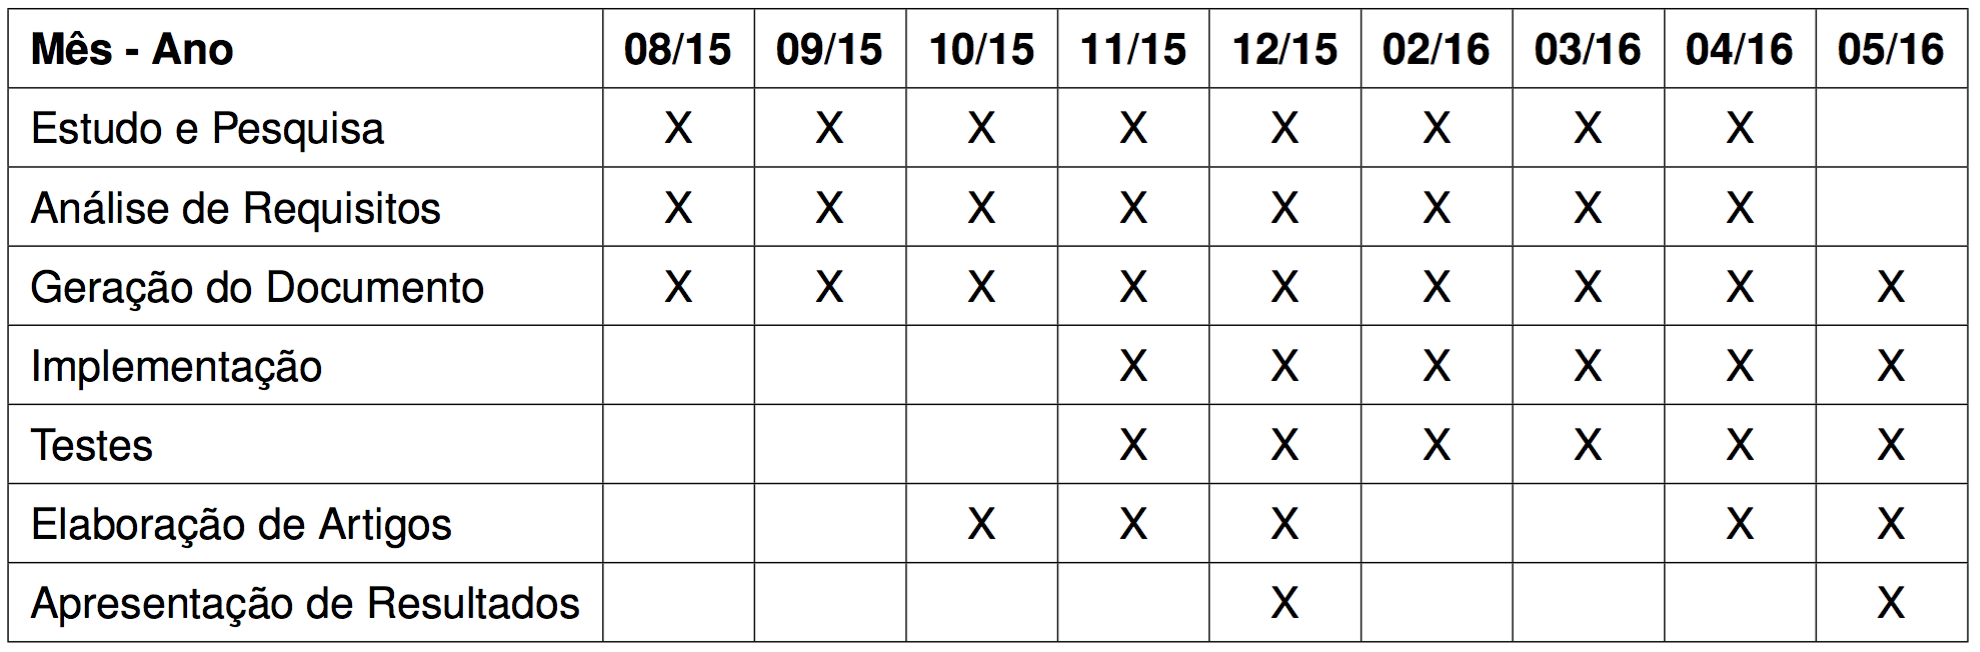
\includegraphics[width=1\textwidth]{Cap1/imagens/tabela}
%%	\vspace{-0.3cm}
%	\legend{FONTE: Elaborado pelo autor}
%	\label{cronograma}
%\end{table}

\begin{table}[h!]
	\centering
	\caption{Cronograma de execução}
	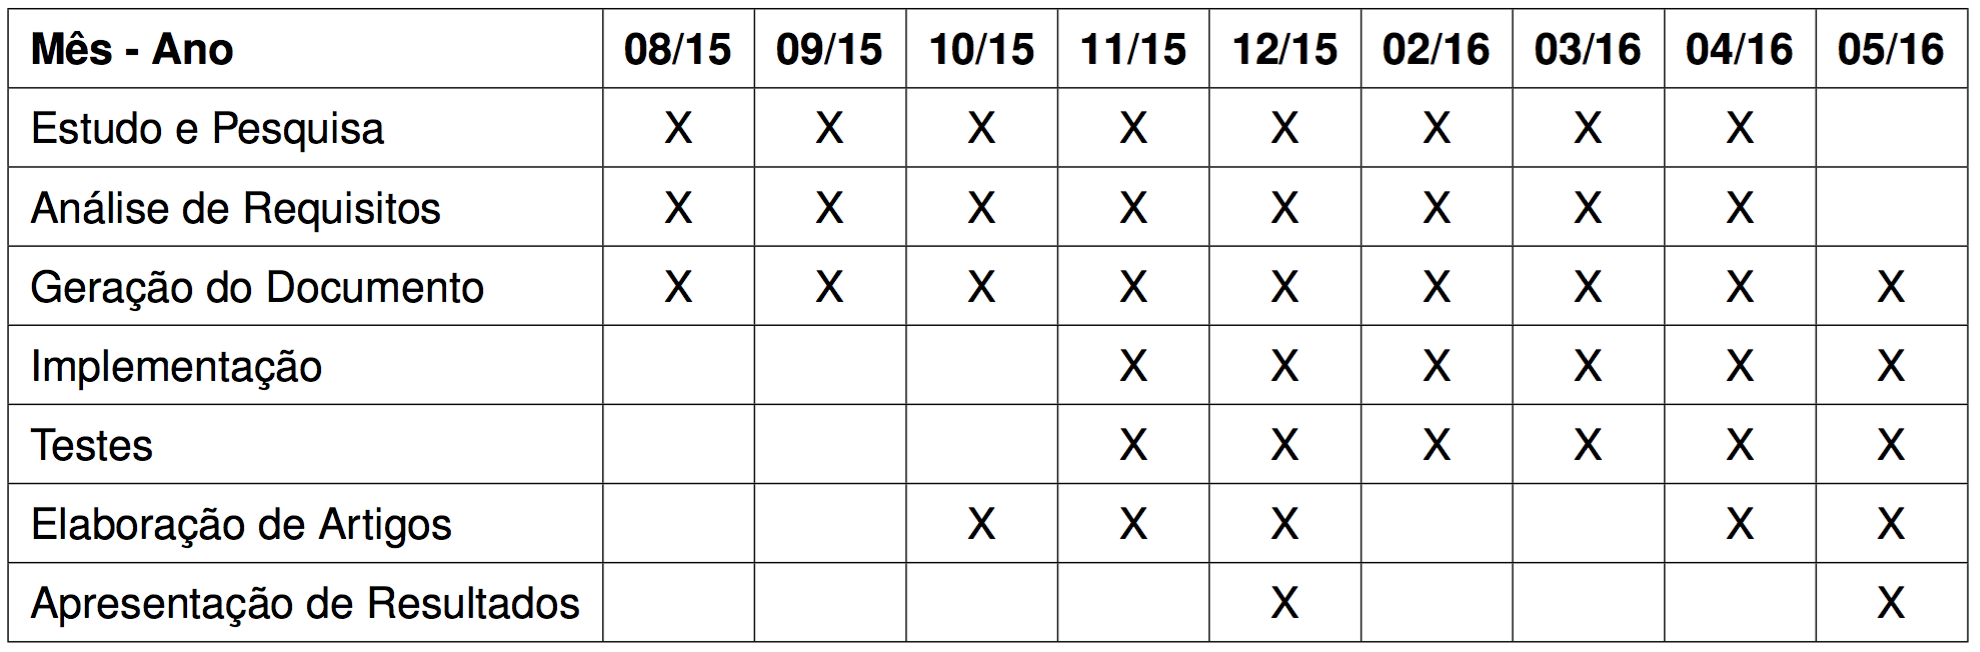
\includegraphics[width=1\textwidth]{Cap1/imagens/tabela}
	\fonte{Elaborado pelo autor}
	\label{cronograma}
\end{table}


\section{ORGANIZAÇÃO DO TRABALHO}\label{sec:organizacao-trabalho}

Além deste capítulo introdutório, este trabalho é composto de mais seis capítulos.

O Capítulo 2 apresenta os trabalhos que são referências para este estudo.

Os fundamentos teóricos, como os conceitos de \textit{data mining} e base para o entendimento do tema proposto, estão descritos no Capítulo 3.

As bibliotecas da linguagem Python utilizadas para a mineração de dados são expostas no Capítulo 4. Também, são apresentadas neste capítulo a API do \textit{Twitter}, as etapas de \textit{data mining} e outros materiais e metodologias utilizados para execução deste trabalho.

No Capítulo 5 são demonstradas as fases do desenvolvimento e implementação de \textit{scripts} para a coleta e obtenção de resultados.

Os resultados obtidos e a apresentação de gráficos e imagens das soluções desenvolvidas são apresentados no Capítulo 6.

Por fim, a conclusão deste trabalho se dá no Capítulo 7, onde são abordadas e analisadas as dificuldades, além de determinar as possibilidades para trabalhos futuros.
